\chapter{Architecture}

In this section we introduce the general architecture of our wrapper for MonPoly.
A more in depth look at the specific technical implementation will be provided in the implementation section.
In general, we have three components for this project.
On one hand we have the MonPoly with a few extensions.
On the other hand is QuestDB.
Our wrapper acts as the glue between the two.
In addition the wrapper also provides a new interface to MonPoly in the form of a REST API.
Figure \ref{fig:wrapper} shows the structure of the MonPoly wrapper.

\begin{figure}
  \centering
  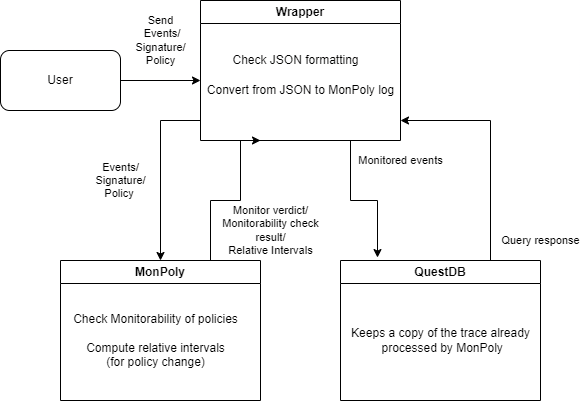
\includegraphics[width=110mm]{diagrams/wrapper.png}
  \caption{Illustration of the project structure}
  \label{fig:wrapper}
\end{figure}


\section{Wrapper}

The wrapper can be run directly on a system with MonPoly installed.
The alternative and more portable way to run it is with a Docker container.
For Docker, the MonPoly Docker image is used as a base image and then the wrapper code and the required Python libraries are installed on top.
In the end the wrapper is simply run like any Flask app.

A QuestDB instance must be running separately.
This can be on the same system locally or somewhere on a remote server.
The connection details for QuestDB, like ports, username, database password, and hostname must be configured in the wrapper for it to be fully operational.

On a high level the user first provides the connection information for the database.
Next a policy and a signature must be sent to the wrapper.
If the signature and policy are monitorable, the user can issue a command to start the monitor and from this point onward the wrapper will accept and process incoming events.

At any point the user can issue a policy change by sending the appropriate command and the new policy.
The wrapper will then perform the policy change and report once it is complete.

\section{The REST API}

In this section we provide a list of all the REST API endpoints, describe their purpose, and give some basic usage examples.

\begin{itemize}
    \item \texttt{/}
    This endpoint is designed to be viewed in the browser, and it displays basic information about the state of the wrapper.
    It shows the current policy and signature, if they have been set.
    Perhaps most importantly it displays the output from MonPoly.

    \item \texttt{/set-policy}
    This takes any policy or formula file for MonPoly.
    At this point no checks on the policy file are performed.
    A monitorability check is only done once both, a policy and a signature, have been set, and the user attempts to start the monitor with \texttt{/start-monitor}.
    For convenience a separate endpoint that does not start the monitor, but performs the monitorability check could be provided.
    Through the optional \texttt{negate} form key, the user can specify whether the negated or non-negated policy should be monitored.
    For this any value provided along with the \texttt{negate} key gets ignored.
    Se the following snippet for how \texttt{/set-policy} could be used with the command line tool curl \cite{curl}.

    \begin{verbatim}
$ curl -X POST -F policy=@<path/to/policy> [-F negate=]
                <wrapper-hostname>[:port]/set-policy
> {"message":"policy set to  <contents of policy file>"}
    \end{verbatim}

    \item \texttt{/set-signature}
    This works very similarly to \texttt{/set-policy}, except it has no optional parameters like \texttt{negate} and as its name describes, it sets the signature and not the policy.
    \begin{verbatim}
$ curl -X POST -F signature=@<path/to/signature> \
                <wrapper-hostname>[:port]/set-signature

{"message":"signature set to <contents of signature file>"}
    \end{verbatim}

    \item \texttt{/start-monitor}
    With this the user can start the monitoring process.
    If either a policy or signature file has not been set yet, this gets reported to the user and the command exits.
    First a monitorability check with the provided policy and signature files is done.
    Any potential issues get reported back.
    When everything is fine, a MonPoly subprocess gets launched and the wrapper is then ready to accept and process incoming events.
    It is worth noting that until the monitor gets started the first time, the policy as well as the signature can be changed freely.
    Passing the \texttt{existing-db} argument along with this command restores the state of the monitor according to potential database entries.
    This can be used, when moving the wrapper from one machine to another.
    With this command the monitor can also be restarted on the same machine if it was stopped properly, e.g. using the \texttt{/stop-monitor} command, and the monitor state was saved to disk.
    Below we illustrate the basic usage for the command along with a sample response for when the command succeeds.
    \begin{verbatim}
$ curl -X GET [-F existing-db=] <wrapper-hostname>[:port]/start-monitor 
{
    "pid": <process id of MonPoly>,
    "args": [ <command line arguments passed to MonPoly> ]
}
    \end{verbatim}

    \item \texttt{/stop-monitor}
    This command stops the MonPoly subprocess in a controlled manner.
    It waits for any processing to be done and then attempts to stop MonPoly with its \texttt{save\_and\_exit } command, which stores the memory state of MonPoly to disk.


    \item \texttt{/change-policy}
    The policy change endpoint can only be used when MonPoly is already running.
    Its usage is analogous to \texttt{set-policy}, as can be seen in the following.
    \begin{verbatim}
$ curl -X POST -F policy=@<path/to/policy> [-F negate=]
                <wrapper-hostname>[:port]/change-policy
> {"success":"changed policy from  <previous policy> to <new policy>"}
    \end{verbatim}
    The inner workings are of course different from those of \texttt{set-policy}.
    We describe these further in the chapters on algorithms and the implementation.
    From a user perspective it is important to know that this command only has an effect on the monitor if the newly provided policy is monitorable against the existing signature.
    If not, the wrapper simply reports any potential issues back to the user and continues monitoring the old policy.
    An important note is that there is no way to change the signature once MonPoly has been started.
    \item \texttt{/get-policy} and \texttt{/get-signature}.
    These command retrieve the monitored policy or signature respectively.
    If no policy or signature has been set yet, the returned value instead of the policy or signature is a string informing the user of that.
    These commands can be used like so:
    \begin{verbatim}
$ curl -X GET localhost:5000/get-policy
> {"policy":"<current policy"}

$ curl -X GET localhost:5000/get-signature
> {"signature":"<current signature"}
    \end{verbatim}

    \item \texttt{/reset-everything}
    This is a destructive command.
    In a real world context this should be used exceedingly rarely.
    It stops any running sub-processes, deletes or resets any configuration files, and clears the database.
    \begin{verbatim}
$ curl -X GET <wrapper-hostname>[:port]/reset-everything
> {
    "config":"deleted <path/to/config/file>",
    "query":<SQL query used to drop tables>,
    "stopped":"stopped monpoly"
  }
    \end{verbatim}
    \item \texttt{/log-events}
    This is perhaps the most important endpoint.
    It is certainly the one that will be used the most as it is the one handling incoming events.
    This command takes as an argument a JSON file with a list of one or more, ordered, time points.
    These time points can optionally have a time stamp associated with them.
    For time points with no specified time stamp the wrapper assigns all them the same time stamp corresponding to the current system time.
    The list does not technically have to be sorted, but any out of order time points will be skipped.
    Time points might also be skipped if they contain predicates with unknown names, a wrong number of attributes, or the wrong types of attributes.
    Time points that are skipped are reported back to the user along with the reason as to why they were skipped.
    We aimed for a high fault tolerance in this regard.
    If some time points in a log file get skipped, they have no effect on the processing of time points that were in order and correctly formatted.
    \begin{verbatim}
$ curl -X POST -F events=@<path/to/JSON/log/file> \
                    <wrapper-hostname>[:port]/log-events        
> {"skipped-timepoints":<dictionary of any skipped time points>}
    \end{verbatim}
    Here we quickly describe our JSON format and how it corresponds to a MonPoly log with the help of a short example in Figure \ref{fig:example-log-monpoly}.
    Consider the following potential log for our ongoing example with the signature from Figure \ref{fig:example-signature}.
\begin{figure}
    \label{fig:example-log-monpoly}
\begin{verbatim}
@10
loc_accessed(2, "advertising") (3, "navigation")

@20
perm_granted(2)
loc_accessed(4, "fitness-tracking")
perm_revoked(3)

@35

@40
perm_revoked(2)
\end{verbatim}
    \caption{Example Log in MonPoly format}
\end{figure}
The same log in our JSON format can be seen in Figure \ref{fig:example-log-json}.
Note that in JSON we have opted for the more human-readable version of a time stamp in Unix format, whereas MonPoly internally always works with integers.
Though MonPoly does provide a flag with which time stamps are displayed to the user in Unix format, for example when a policy violation occurs at a time point.
\begin{figure}
    \label{fig:example-log-json}
\begin{verbatim}
[
    {
        "timestamp": "1970-01-01 00:00:10",
        "predicates": [
            {
                "name": "loc_accessed",
                "occurrences": [
                    [2, "advertising"], [3, "navigation"]
                ]
            }
        ]
    },
    {
        "timestamp": "1970-01-01 00:00:20",
        "predicates": [
            {
                "name": "loc_accessed",
                "occurrences": [
                    [4, "fitness-tracking"]
                ]
            },
            {
                "name": "perm_granted",
                "occurrences": [
                    [2]
                ]
            },
            {
                "name": "perm_revoked",
                "occurrences": [
                    [3]
                ]
            }
        ]
    },
    {
        "timestamp": "1970-01-01 00:00:35",
        "predicates": []
    },
    {
        "timestamp": "1970-01-01 00:00:35",
        "predicates": [
            {
                "name": "perm_revoked",
                "occurrences": [
                    [2]
                ]
            }
        ]
    }
]
\end{verbatim}
    \caption{Example Log in JSON format}
\end{figure}

    \item \texttt{/get-events}
    This endpoint is a direct interface to the database and queries all time points in a specified time range.
    The time range can be specified with optional \texttt{start} and \texttt{end} parameters.
    These parameters should be formatted just like the time stamps in our JSON log files.
    The time points get returned in the same JSON format as described above.

    \begin{verbatim}
$ curl -X GET [-F start=<start-date>] [-F end=<end-date>] \
               <wrapper-hostname>[:port]/get-events
> [<list of all time points with their events>]
    \end{verbatim}

    \item \texttt{/get-most-recent}
    This command simply returns the latest time point that is stored in the database.
    If the database is still empty, the returned value is simply \texttt{null}.
    \begin{verbatim}
$ curl -X GET <wrapper-hostname>[:port]/get-most-recent
> {"response": <time stamp of newest time point, or null>}
    \end{verbatim}


\end{itemize}

The wrapper also provides various "getter"- and "setter"- methods for the configuration details of QuestDB.
They do not change the configuration of QuestDB itself, but simply tell the wrapper how to reach QuestDB.
These should be fairly self-explanatory.
We will quickly list them here for completeness. 
For more information on what each of these values does, the QuestDB documentation \cite{questdb,questdb-postgres-wire,questdb-influx-db-line-protocol} can be consulted.
The QuestDB related endpoints are:\\
\texttt{/db-set-user}, \\
\texttt{/db-set-password}, \\
\texttt{/db-set-host}, \\
\texttt{/db-set-pgsql-port}, \\
\texttt{/db-set-influxdb-port}, \\
\texttt{/db-set-database}, \\
\texttt{/db-get-user}, \\
\texttt{/db-get-password}, \\
\texttt{/db-get-host}, \\
\texttt{/db-get-pgsql-port},\\
\texttt{/db-get-influxdb-port}, and \\
\texttt{/db-get-database}.






